% Options for packages loaded elsewhere
\PassOptionsToPackage{unicode}{hyperref}
\PassOptionsToPackage{hyphens}{url}
\PassOptionsToPackage{dvipsnames,svgnames,x11names}{xcolor}
%
\documentclass[
]{article}
\usepackage{booktabs}
\usepackage{url}
\usepackage{amsmath,amssymb}
\usepackage{lmodern}
\usepackage{iftex}
\usepackage{listings}
\usepackage{xcolor}
\usepackage{float}
\ifPDFTeX
  \usepackage[T1]{fontenc}
  \usepackage[utf8]{inputenc}
  \usepackage{textcomp} % provide euro and other symbols
\else % if luatex or xetex
  \usepackage{unicode-math}
  \defaultfontfeatures{Scale=MatchLowercase}
  \defaultfontfeatures[\rmfamily]{Ligatures=TeX,Scale=1}
\fi
% Use upquote if available, for straight quotes in verbatim environments
\IfFileExists{upquote.sty}{\usepackage{upquote}}{}
\IfFileExists{microtype.sty}{% use microtype if available
  \usepackage[]{microtype}
  \UseMicrotypeSet[protrusion]{basicmath} % disable protrusion for tt fonts
}{}
\makeatletter
\@ifundefined{KOMAClassName}{% if non-KOMA class
  \IfFileExists{parskip.sty}{%
    \usepackage{parskip}
  }{% else
    \setlength{\parindent}{0pt}
    \setlength{\parskip}{6pt plus 2pt minus 1pt}}
}{% if KOMA class
  \KOMAoptions{parskip=half}}
\makeatother
\usepackage{xcolor}
\usepackage{graphicx}
\usepackage{natbib}
\makeatletter
\def\maxwidth{\ifdim\Gin@nat@width>\linewidth\linewidth\else\Gin@nat@width\fi}
\def\maxheight{\ifdim\Gin@nat@height>\textheight\textheight\else\Gin@nat@height\fi}

\lstdefinestyle{mystyle}{
    language=Python,
    basicstyle=\ttfamily\small,
    commentstyle=\color{gray},
    keywordstyle=\color{blue},
    numberstyle=\tiny\color{gray},
    stringstyle=\color{red},
    breakatwhitespace=false,         
    breaklines=true,                 
    captionpos=b,                    
    keepspaces=true,                 
    numbers=left,                    
    numbersep=5pt,                  
    showspaces=false,                
    showstringspaces=false,
    showtabs=false,                  
    tabsize=2
}
\lstset{style=mystyle}
\makeatother
% Scale images if necessary, so that they will not overflow the page
% margins by default, and it is still possible to overwrite the defaults
% using explicit options in \includegraphics[width, height, ...]{}
\setkeys{Gin}{width=\maxwidth,height=\maxheight,keepaspectratio}
% Set default figure placement to htbp
\makeatletter
\def\fps@figure{htbp}
\makeatother
\setlength{\emergencystretch}{3em} % prevent overfull lines
\providecommand{\tightlist}{%
  \setlength{\itemsep}{0pt}\setlength{\parskip}{0pt}}
\setcounter{secnumdepth}{-\maxdimen} % remove section numbering
% definitions for citeproc citations
\NewDocumentCommand\citeproctext{}{}
\NewDocumentCommand\citeproc{mm}{%
  \begingroup\def\citeproctext{#2}\cite{#1}\endgroup}
\makeatletter
 % allow citations to break across lines
 \let\@cite@ofmt\@firstofone
 % avoid brackets around text for \cite:
 \def\@biblabel#1{}
 \def\@cite#1#2{{#1\if@tempswa , #2\fi}}
\makeatother
\newlength{\cslhangindent}
\setlength{\cslhangindent}{1.5em}
\newlength{\csllabelwidth}
\setlength{\csllabelwidth}{3em}
\newenvironment{CSLReferences}[2] % #1 hanging-indent, #2 entry-spacing
 {\begin{list}{}{%
  \setlength{\itemindent}{0pt}
  \setlength{\leftmargin}{0pt}
  \setlength{\parsep}{0pt}
  % turn on hanging indent if param 1 is 1
  \ifodd #1
   \setlength{\leftmargin}{\cslhangindent}
   \setlength{\itemindent}{-1\cslhangindent}
  \fi
  % set entry spacing
  \setlength{\itemsep}{#2\baselineskip}}}
 {\end{list}}
\usepackage{calc}
\newcommand{\CSLBlock}[1]{\hfill\break\parbox[t]{\linewidth}{\strut\ignorespaces#1\strut}}
\newcommand{\CSLLeftMargin}[1]{\parbox[t]{\csllabelwidth}{\strut#1\strut}}
\newcommand{\CSLRightInline}[1]{\parbox[t]{\linewidth - \csllabelwidth}{\strut#1\strut}}
\newcommand{\CSLIndent}[1]{\hspace{\cslhangindent}#1}
\ifLuaTeX
\usepackage[bidi=basic]{babel}
\else
\usepackage[bidi=default]{babel}
\fi
\babelprovide[main,import]{american}
% get rid of language-specific shorthands (see #6817):
\let\LanguageShortHands\languageshorthands
\def\languageshorthands#1{}
\ifLuaTeX
  \usepackage{selnolig}  % disable illegal ligatures
\fi
\IfFileExists{bookmark.sty}{\usepackage{bookmark}}{\usepackage{hyperref}}
\IfFileExists{xurl.sty}{\usepackage{xurl}}{} % add URL line breaks if available
\urlstyle{same} % disable monospaced font for URLs
\hypersetup{
  pdftitle={LangFair: A Python Package for Assessing Bias and Fairness in Large Language Model Use Cases},
  pdfauthor={Bouchard et al.},
  pdflang={en-US},
  colorlinks=true,
  linkcolor={Maroon},
  filecolor={Maroon},
  citecolor={Blue},
  urlcolor={Blue},
  pdfcreator={LaTeX via pandoc}}

\title{LangFair: A Python Package for Assessing Bias and Fairness in Large Language Model Use Cases}


%%%%%%%%%%%%%%%%%%%%%%%%%%%%%%%%%%%%%%%%%%%%%%%%%%%%%%%%%%%%%%%%%%%%%%%%
% Authors and Affiliations

\usepackage[affil-it]{authblk}
\usepackage{orcidlink}
%% \renewcommand\Authsep{, }
\setlength{\affilsep}{1em}
\author[1]{Dylan Bouchard%
    \,\orcidlink{0009-0004-9233-2324}\,%
    }

\author[1]{Mohit Singh Chauhan%
    \,\orcidlink{0000-0002-7817-0427}\,%
    }

\author[1]{David Skarbrevik%
    \,\orcidlink{0009-0005-0005-0408}\,%
    }

\author[1]{Viren Bajaj%
    \,\orcidlink{0000-0002-9984-1293}\,%
    }

\author[1]{Zeya Ahmad%
    \,\orcidlink{0009-0009-1478-2940}\,%
    }

\affil[1]{CVS Health\textsuperscript{\textregistered} Corporation}
%%%%%%%%%%%%%%%%%%%%%%%%%%%%%%%%%%%%%%%%%%%%%%%%%%%%%%%%%%%%%%%%%%%%%%%%
\date{1 June 2024}

\begin{document}
\maketitle


\section{Summary}

Large Language Models (LLMs) have been observed to exhibit bias in numerous ways, potentially creating or worsening outcomes for specific groups identified by protected attributes such as sex, race, sexual orientation, or age. The versatile capabilities of contemporary LLMs in executing a range of tasks, as highlighted in recent studies \cite{minaee2024large, chatgpt_survey, generalsurvey}, pose significant challenges in assessing bias and fairness at the model level.

To help address this gap, we introduce LangFair, an open-source initiative that aims to equip LLM practitioners with the tools to evaluate bias and fairness risks relevant to their specific use cases. This evaluation method is distinctive as it incorporates actual prompts from the practitioner's use case, offering a customized assessment that accounts for prompt-specific risks that have been shown to substantially increase the probability of biased and unfair outcomes \cite{wang2023decodingtrust}. While a comprehensive discussion of selection of bias and fairness metrics is outside the scope of this paper, we direct the reader to our companion paper, \cite{bouchard2024actionableframeworkassessingbias}, for further details.

This paper details the accompanying Python library, \texttt{langfair}, which enables practitioners to implement the aforementioned framework in a low-code, user-friendly fashion.\footnote{The repository for \texttt{langfair} can be found at \url{https://github.com/cvs-health/langfair}.} The library offers functionality to easily generate evaluation datasets, comprised of LLM responses to use-case-specific prompts, and subsequently calculate applicable metrics for the practitioner's use case. Following \cite{bouchard2024actionableframeworkassessingbias}, evaluation metrics are categorized according to the risks they assess (toxicity, stereotypes, counterfactual unfairness, and allocational harms), as well as the use case task (text generation, classification, and recommendation).\footnote{Note that text generation encompasses all use cases for which output is text, but does not belong to a predefined set of elements (as with classification and recommendation).}





\section{Statement of Need}
Traditional machine learning (ML) fairness toolkits like AIF360 \cite{aif360-oct-2018}, Fairlearn \cite{Weerts_Fairlearn_Assessing_and_2023}, Aequitas \cite{2018aequitas} and others \cite{lift,DBLP:journals/corr/abs-1907-04135,tensorflow-no-date} have laid crucial groundwork but are not tailored to the generative and context-dependent nature of LLMs.

LLMs are used in systems that solve tasks such as recommendation, classification, text generation, and summarization. In practice, these systems try to restrict the responses of the LLM to the task at hand, often by including task-specific instructions in system or user prompts. When the LLM is evaluated without taking the set of task-specific prompts into account, the evaluation metrics are not representative of the system's true performance. Representing the system's actual performance is especially important when evaluating its outputs for bias and fairness risks because they pose real harm to the user and, by way of repercussions, the system developer.

Most evaluation tools, including those that assess bias and fairness risk, evaluate LLMs at the model-level by calculating metrics based on the responses of the LLMs to static benchmark datasets of prompts \cite{rudinger-EtAl:2018:N18,zhao-2018,vnmssnhv-no-date,webster2018gap, levy2021collecting,nadeem2020stereoset,bartl2020unmasking,nangia2020crows,katyfelkner-no-date,umanlp-no-date,unknown-author-no-date,dev2019measuring,Gehman2020RealToxicityPromptsEN,bold_2021,smith2022imsorry,howiehwong-no-date,nozza-etal-2021-honest,nyu-mll-no-date,li2020unqover,krieg2022grep} that do not consider prompt-specific risks and are often independent of the task at hand. Holistic Evaluation of Language Models (HELM) \cite{liang2023holisticevaluationlanguagemodels},DecodingTrust \cite{wang2023decodingtrust}, and several others \cite{srivastava2023beyond,huang2024trustllm,eval-harness} follow this paradigm. Some tools allow you to configure the evaluation to specific but predefined tasks such as LightEval \cite{lighteval}, langtest \cite{Arshaan_Nazir_and_Thadaka_Kalyan_Chakravarthy_and_David_Amore_Cecchini_and_Thadaka_Kalyan_Chakravarthy_and_Rakshit_Khajuria_and_Prikshit_Sharma_and_Ali_Tarik_Mirik_and_Veysel_Kocaman_and_David_Talby_LangTest_A_comprehensive_2024}, and others \cite{confident-ai-no-date,giskard-ai-no-date,huggingface-no-date}. 

LangFair complements the aforementioned frameworks because it follows a bring your own prompts (BYOP) approach, which allows users to tailor the bias and fairness evaluation to their use case by computing metrics using LLM responses to user-provided prompts. This addresses the need for a task-based bias and fairness evaluation tool that accounts for prompt-specific risk for LLMs.\footnote{Experiments in \cite{wang2023decodingtrust} demonstrate that prompt content has substantial influence on the likelihood of biased LLM responses.}


LangFair addresses another challenge faced by developers: navigating the large number of bias and fairness metrics to find the ones that apply to their use case. While the aforementioned collection of existing tools offer extensive metric coverage, LangFair offers an actionable decision framework to guide metric selection \cite{bouchard2024actionableframeworkassessingbias}. The package is designed based on this decision framework to derive metrics that are applicable to recommendation, classification, and text generation tasks based on use-case-specific properties such as fairness through unawareness \cite{gallegos2024biasfairnesslargelanguage}, inputs corresponding to protected attribute groups, etc. 

Furthermore, LangFair is designed for real-world LLM-based systems that require governance audits. LangFair focuses on calculating metrics from LLM responses only, which is more practical for real-world testing where access to internal states of model to retrieve embeddings or token probabilities is difficult. An added benefit is that output-based metrics, which are focused on the downstream task, have shown to be potentially more reliable than metrics derived from embeddings or token probabilities \cite{intrinsic_do_not, biased_rulers}.




\section{Generation of Evaluation Datasets}
Following \cite{bouchard2024actionableframeworkassessingbias}, we define bias and fairness assessments for LLMs on a use case level. Under this approach, evaluation metrics are computed on a set of LLM responses generated from prompts sampled from the use case's population of prompts. Accordingly, the \texttt{langfair.generator} module offers two classes, \texttt{ResponseGenerator} and \texttt{CounterfactualGenerator}, which aim to enable user-friendly construction of evaluation datasets for text generation use cases.


\paragraph{\texttt{ResponseGenerator} class.}
To streamline generation of evaluation datasets, the \texttt{ResponseGenerator} class wraps an instance of a \texttt{langchain} LLM and leverages asynchronous generation with \texttt{asyncio}. Users should customize the \texttt{langchain} LLM instance to match the parameters of the use case being assessed. To implement, users simply pass a list of prompts (strings) to the \texttt{ResponseGenerator.generate\_responses} method, which returns a dictionary containing prompts, responses, and applicable metadata. In addition, the \texttt{ResponseGenerator.estimate\_token\_cost} method enables users to estimate the approximate cost of generation with select \texttt{OpenAI} models in advance by counting tokens with the \texttt{tiktoken} library. In particular, \texttt{tiktoken} and model-cost mapping are used to a) compute deterministic input token costs from a provided list of prompts and b) estimate stochastic output token costs from a sample of generated responses.\footnote{Token costs for select OpenAI models are obtained from \url{https://openai.com/api/pricing/}.}

\paragraph{\texttt{CounterfactualGenerator} class.}
Counterfactual fairness assessments are recommended \cite{huang2020reducingsentimentbiaslanguage, bouchard2024actionableframeworkassessingbias} for text generation use cases that do not satisfy fairness through unawareness (FTU), i.e., prompts contain mentions of protected attribute information \cite{gallegos2024biasfairnesslargelanguage}. In the context of LLMs, counterfactual fairness can be assessed by constructing counterfactual input pairs \cite{gallegos2024biasfairnesslargelanguage, bouchard2024actionableframeworkassessingbias}, comprised of prompt pairs that mention different protected attribute groups but are otherwise identical, and measuring the differences in the corresponding generated output pairs. 


A subclass of \texttt{ResponseGenerator}, the \texttt{CounterfactualGenerator} offers functionality to check for FTU, construct counterfactual input pairs, and generate corresponding pairs of responses asynchronously using a \texttt{langchain} LLM instance. Off the shelf, the FTU check and creation of counterfactual input pairs can be done for gender and race/ethnicity, but users may also provide a custom mapping of protected attribute words to enable this functionality for other attributes as well.\footnote{For instance, one example of a custom counterfactual mapping could be \texttt{\{'old': ['old', 'elderly', 'senior'], 'young': ['young', 'youthful', 'juvenile']\}.}} To construct the counterfactual input pairs, token-based substitution is conducted on user-provided prompts. For instance, the input prompt \texttt{`the husband went to the store'}, would yield the counterfactual input pair \texttt{[`the husband went to the store', `the wife went to the store']} for gender.


\section{Bias and Fairness Evaluations for Focused Use Cases}
The evaluation metrics supported by LangFair assess the following bias and fairness risks: toxicity, stereotypes, counterfactual (un)fairness, and allocational harms. Table \ref{tab:metrics} maps the classes contained in the \texttt{langfair.metrics} module to these risks. These classes are discussed in detail below.


\begin{table}[H]
\centering
\caption{Classes for Computing Evaluation Metrics in \texttt{langfair.metrics}}
\label{tab:metrics}
\begin{tabular}{lll}
Class                                           & Risk Assessed             & Applicable Tasks           \\
\toprule
\texttt{ToxicityMetrics}       & Toxicity                  & Text generation \\
\texttt{StereotypeMetrics}     & Stereotypes               & Text generation \\
\texttt{CounterfactualMetrics} & Counterfactual fairness & Text generation \\
\texttt{RecommendationMetrics} & Counterfactual fairness & Recommendation  \\
\texttt{ClassificationMetrics} & Allocational harms        & Classification  \\     
\bottomrule
\end{tabular}
\end{table}


\paragraph{Toxicity Metrics}
The \texttt{ToxicityMetrics} class facilitates simple computation of toxicity metrics from a user-provided list of LLM responses. These metrics include \textit{expected maximum toxicity} \cite{Gehman2020RealToxicityPromptsEN}, \textit{toxicity probability} \cite{Gehman2020RealToxicityPromptsEN}, and \textit{toxic fraction} \cite{liang2023holisticevaluationlanguagemodels}, all of which leverage a pre-trained toxicity classifier that maps a text input to a toxicity score ranging from 0 to 1. For off-the-shelf toxicity classifiers, the \texttt{ToxicityMetrics} class provides four options: two classifiers from the \texttt{detoxify} package, \texttt{roberta-hate-speech-dynabench-r4-target} from the \texttt{evaluate} package, and \texttt{toxigen} available on HuggingFace.\footnote{\url{https://github.com/unitaryai/detoxify}}\footnote{\url{https://github.com/huggingface/evaluate}}\footnote{\url{https://github.com/microsoft/TOXIGEN}} For additional flexibility, users can specify an ensemble of the off-the-shelf classifiers offered or provide a custom toxicity classifier object. 

\paragraph{Stereotype Metrics}
LLMs have been observed to include harmful stereotypes in their generated responses \cite{liang2023holisticevaluationlanguagemodels, bordia-bowman-2019-identifying, zekun2023auditinglargelanguagemodels}. To measure stereotypes in LLM responses, the \texttt{StereotypeMetrics} class offers two classes of metrics: metrics based on word cooccurrences and metrics that leverage a pre-trained stereotype classifier. In particular, metrics based on word cooccurrences include \textit{cooccurrence bias score} \cite{bordia-bowman-2019-identifying} and \textit{stereotypical associations} \cite{liang2023holisticevaluationlanguagemodels} and aim to assess relative cooccurrence of stereotypical words with certain protected attribute words. Stereotype classifier metrics leverage the \texttt{wu981526092/Sentence-Level-Stereotype-Detector} classifier available on HuggingFace \cite{zekun2023auditinglargelanguagemodels} and compute analogs of the aforementioned toxicity classifier metrics \cite{bouchard2024actionableframeworkassessingbias}.\footnote{\url{https://huggingface.co/wu981526092/Sentence-Level-Stereotype-Detector}}

\paragraph{Counterfactual Fairness Metrics for Text Generation}
 The \texttt{CounterfactualMetrics} class offers two groups of metrics to assess counterfactual fairness in text generation use cases. The first set of metrics leverage a pre-trained sentiment classifier to measure sentiment disparities in counterfactually generated outputs \cite{huang2020reducingsentimentbiaslanguage, bouchard2024actionableframeworkassessingbias}. This class uses the \texttt{vaderSentiment} classifier by default but also gives users the option to provide a custom sentiment classifier object.\footnote{\url{https://github.com/cjhutto/vaderSentiment}} The second group of metrics addresses a stricter desiderata and measures overall similarity in counterfactually generated outputs. Following \cite{bouchard2024actionableframeworkassessingbias}, these metrics apply well-established text similarity metrics including \textit{recall-oriented understudy for gisting evaluation} (\textit{ROUGE}) \cite{lin-2004-rouge}, \textit{bilingual evaluation understudy} (\textit{BLEU}) \cite{10.3115/1073083.1073135}, and \textit{cosine similarity} to measure counterfactual similarity.


\paragraph{Counterfactual Fairness Metrics for Recommendation}
When LLMs are used for recommendation, they pose the risk of discriminating when exposed to protected attribute information in input prompts \cite{Zhang_2023}. To assess counterfactual fairness for recommendation use cases, the \texttt{RecommendationMetrics} class offers three metrics, proposed by \cite{Zhang_2023}. Specifically, for counterfactually generated sets of $K$ recommendations, these metrics include \textit{Jaccard-K}, \textit{pairwise ranking accuracy gap} (\textit{PRAG-K}), and \textit{search result page misinformation score} (\textit{SERP-K}). Metrics may be computed pairwise \cite{bouchard2024actionableframeworkassessingbias}, or attribute-wise \cite{Zhang_2023}.

\paragraph{Fairness Metrics for Classification}
Allocational harms, as measured by group fairness metrics for classification models, has been widely studied in the machine learning fairness literature \cite{2018aequitas, aif360-oct-2018, Weerts_Fairlearn_Assessing_and_2023, feldman2015certifyingremovingdisparateimpact, 10.5555/3120007.3120011, hardt2016equalityopportunitysupervisedlearning, pleiss2017fairnesscalibration, 10.1109/ICDM.2012.45, agarwal2018reductionsapproachfairclassification, zhang2018mitigatingunwantedbiasesadversarial}. When LLMs are used to solve classification problems, traditional machine learning fairness metrics may be applied, provided that inputs can be mapped to a protected attribute. To this end, the \texttt{ClassificationMetrics} class offers a suite of metrics to address unfair classification. Following the framework proposed by \cite{2018aequitas}, metrics are segmented into three categories: representation fairness, error-based fairness for assistive use cases, and error-based fairness for punitive use cases. Representation fairness includes a single metric that measures disparity in predicted prevalence rates \cite{feldman2015certifyingremovingdisparateimpact, 2018aequitas}. For assistive (punitive) classification use cases, metrics measure disparities in false negative rate and false omission rate (false positive rate and false discovery rate).\footnote{In the context of fairness, false negatives are especially costly for use cases that are assistive in nature, e.g. qualifying for a benefits program, . Hence, the recommended metrics for these use cases assess disparities in false negatives across groups. Conversely, false positives are highly costly in punitive use cases (e.g. fraud prediction), and hence the associated metrics focus on disparities in false positives across groups.} When computing metrics using the \texttt{ClassificationMetrics} class, the user may specify whether to compute these metrics as pairwise differences \cite{aif360-oct-2018} or pairwise ratios \cite{2018aequitas}.





\section{Semi-Automated Evaluation}
\paragraph{\texttt{AutoEval} class.} 
To streamline assessments for text generation use cases, the \texttt{AutoEval} class conducts a multi-step process that includes metric selection, evaluation dataset generation, and metric computation. The user is required to supply a list of prompts and an instance of \texttt{langchain} LLM. Below we provide a basic example demonstrating the execution of \texttt{AutoEval.evaluate} with a \texttt{gemini-pro} instance.\footnote{Note that this example assumes the user has already set up their VertexAI credentials and sampled a list of prompts from their use case prompts.}


\begin{lstlisting}[language=Python, caption=\texttt{AutoEval} Example]
from langchain_google_vertexai import VertexAI
from langfair.auto import AutoEval

llm = VertexAI(model_name='gemini-pro')
auto_object = AutoEval(prompts=prompts, langchain_llm=llm)
results = await auto_object.evaluate()
\end{lstlisting}




Under the hood, the \texttt{AutoEval.evaluate} method 1) checks for FTU, 2) generates responses and counterfactual responses (if FTU is not satisfied), and 3) calculates applicable metrics for the use case.\footnote{The \texttt{AutoEval} class is designed specifically for text generation use cases. Applicable metrics include toxicity metrics, stereotype metrics, and, if FTU is not satisfied, counterfactual fairness metrics.} This process flow is depicted in Figure \ref{fig:autoeval_flowchart}.

\begin{figure}[H]
    \centering
    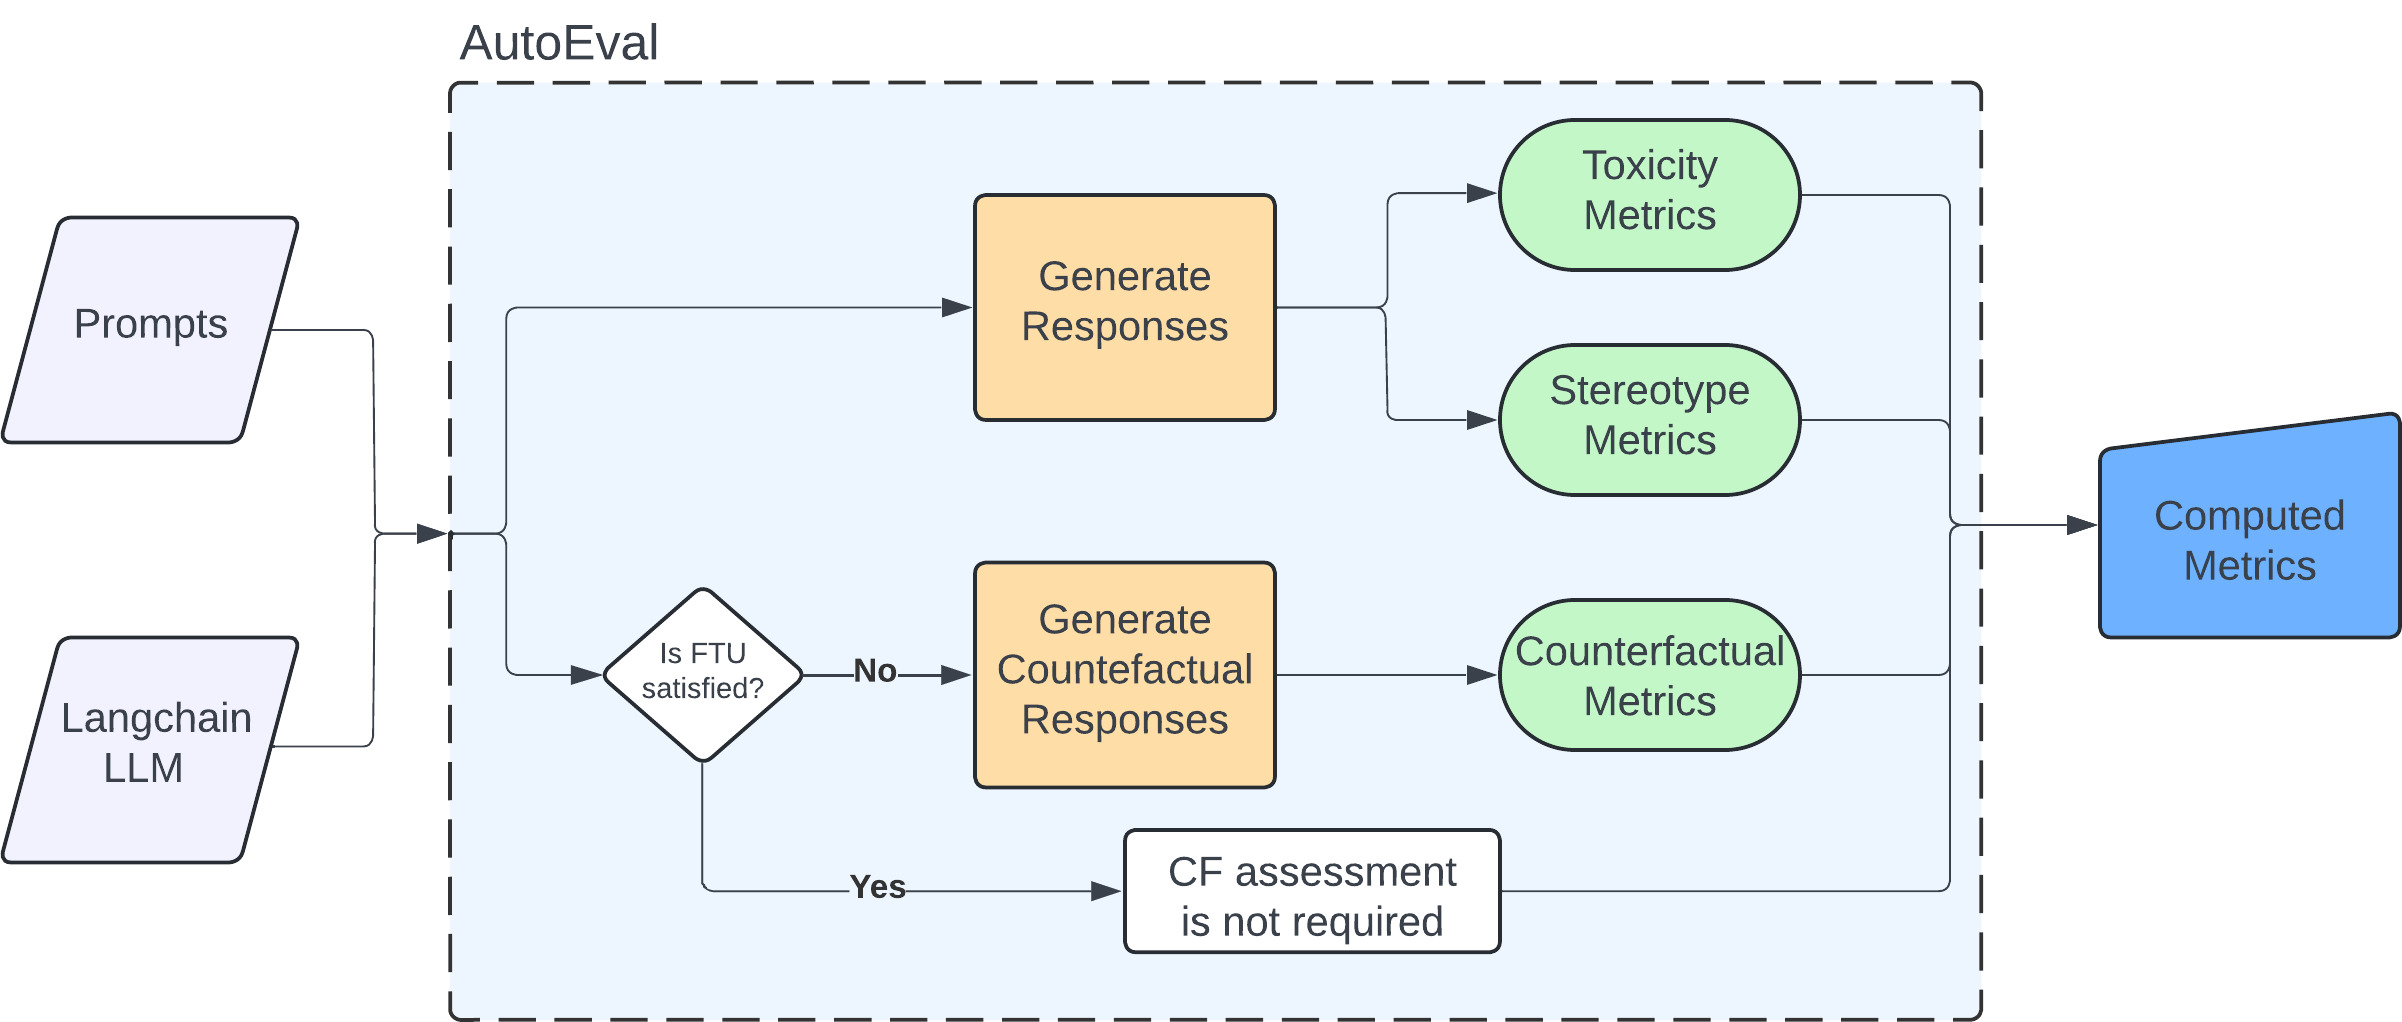
\includegraphics[width=\linewidth]{figures/AutoEval_flowchart_colored.jpeg}
    \caption{Flowchart of internal design of \texttt{AutoEval.evaluate} method.}
    \label{fig:autoeval_flowchart}
\end{figure}




\section*{Author Contributions}
Dylan Bouchard was the principal developer and researcher of the LangFair project, responsible for conceptualization, methodology, and software development of the \emph{langfair} library. Mohit Singh Chauhan was the architect behind the structural design of the \emph{langfair} library and helped lead the software development efforts. David Skarbrevik was the primary author of LangFair's documentation, helped implement software engineering best practices, and contributed to software development. Viren Bajaj wrote unit tests, contributed to the software development, and helped implement software engineering best practices. Zeya Ahmad contributed to the software development. 


\section*{Acknowledgements}
We wish to thank Piero Ferrante, Blake Aber, Xue (Crystal) Gu, and Zirui Xu for their helpful suggestions.

\bibliographystyle{plain}
\bibliography{ref.bib}




\end{document}
